\documentclass[journal]{IEEEtran}

\usepackage{cite}
\usepackage{amsmath}
\interdisplaylinepenalty=2500
\usepackage{algorithm}
\usepackage[noend]{algpseudocode}
\usepackage{array}
\usepackage{graphicx}
\usepackage{float}

% correct bad hyphenation here
\hyphenation{}


\begin{document}
\title{Case Study: Particle Swarm Optimization implementation and comparison}

\author{Wilbert~Pumacay,~\textit{Catholic University San Pablo},~wilbert.pumacay@ucsp.edu.pe\\
        Gerson~Vizcarra,~\textit{Catholic University San Pablo},~gerson.vizcarra@ucsp.edu.pe}

% make the title area
\maketitle

\begin{abstract}
Heuristic-based swarm algorithms emerged as a powerful family of optimization techniques, inspired by the collective behavior of social animals. Particle Swarm Optimization (PSO) , part of this family, is known to solve large-scale nonlinear optimization problems using particles as a set of candidate solutions. In this paper we test the PSO on 3 common benchmarks functions, present a parallel implementation of the algorithm, and compare it with the results from other metaheuristics using the Wilcoxon rank sum test. 
\\
\\
\end{abstract}

\begin{IEEEkeywords}
Metaheuristics, Particle Swarm Optimization, Convergence Behavior, CUDA.
\end{IEEEkeywords}


\section{Introduction}

\IEEEPARstart{T}{he} Particle Swarm Optimization algorithm is a population-based optimization method. It is based on the social behavior of birds and fish when moving as a group.\\

PSO has been applied to many areas such as artificial neural network training, function optimization, fuzzy control, and pattern classification because of its ease of implementation and fast convergence to acceptable solutions.

\section{ Particle Swarm Optimization (PSO) }
\subsection{ Basic concepts }
Particle Swarm Optimization, first introduced by Kennedy and Eberhart \cite{Kennedy1995} is a stochastic optimization technique that is based on two fundamental disciplines·\cite{delValle2008}: social science and computer science. In addition, PSO uses the swarm intelligence concept: the collective behavior of unsophisticated agents that are interacting locally with their environment to create coherent global functional patterns.

\subsection{ Description of the algorithm }
PSO is a population based optimization technique, where the population is called a \textit{swarm}. Earch particle represents a posible solution to the optimization task at hand. During each iteration each particle accelerates in the direction of its own personal best solution found so far, as well as the direction of the global best solution discovered so far by any of the particles in the swarm, as described in Fig. 1. This means that if a particle found a promising new solution, the other particles will move closer to it. The whole algorithm can be described in Algorithm 1.
\\
\begin{figure}[H]
\centering
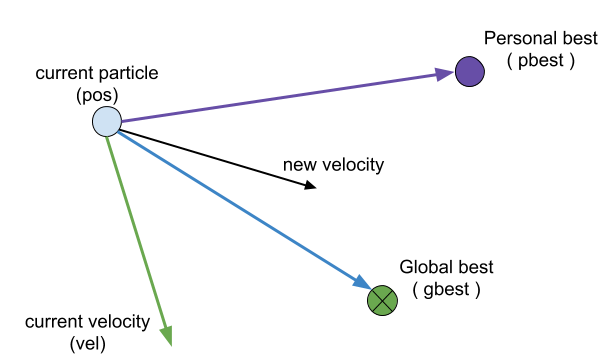
\includegraphics[width=3.0in]{_img/img_PSO_overview.png}
\caption{PSO overview}
\end{figure}

\begin{algorithm}
    \caption{Particle Swarm Optimization Algorithm}\label{alg:PSOpseudocode}
    \begin{algorithmic}[1]
        \State $\textbf{In}: \textit{objFunction, populationSize, w, $c_{1}$, $c_{2}$, k}$
        \State $\textbf{Out}: \textit{Solution optima } P_{g.cost}$
        \State $P_{g.pos} = \textbf{0}$
        \State $P_{g.cost} = Inf$
        \State $particles = \textbf{CreateParticles()}$
        \While {$\textit{ !stopCondition() }$}
            \For {$p$ {\bfseries in} $particles$}
                \State $\textbf{UpdateParticlesVelocities()}$
                \State $\textbf{UpdateParticlesPositions()}$
                \State $\textbf{UpdatePersonalBest()}$
                \State $\textbf{UpdateGlobalBest()}$
            \EndFor
        \EndWhile
        \\
        \Return $P_{g.cost}$
    \end{algorithmic}
\end{algorithm}

Each individual particle has the following attributes: 
\\
\begin{itemize}
    \item A current position in search space $x$.
    \item A current velocity $v$.
    \item A personal best position in the search space $x^{pbest}$.
\end{itemize}
As desribed earlier, each particle updates its velocity according to its personal best and the global best. The update rule (based in the social behaviour mentioned earlier ) can be described with the following equation:
\\
\begin{equation} \label{eq:1}
    \begin{aligned}
    v \leftarrow w v + c_{1} r_{1} [x^{pbest} - x] + c_{2} r_{2} [x^{gbest} - x]
    \end{aligned}
\end{equation}

Where $w$ (inertia coefficient ), $c_{1}$ (cognitive coefficient ), $c_{2}$ (social coefficient ) and $k$ are the hyperparameters of the algorithm; and $r_{1}$ and $r_{2}$ are random numbers in the range $[0, 1]$. We then just update the particle position with the just calculated velocity.

\begin{equation} \label{eq:2}
    \begin{aligned}
        x \leftarrow x + v.
    \end{aligned}
\end{equation}

The personal best position of each particle, $x^{pbest}$ is updated using the following equation :
\begin{equation} \label{eq:3}
  \begin{aligned}
    x^{pbest} \leftarrow x, &&\textit{if } Cost(x)\leq Cost(x^{pbest})
  \end{aligned}
\end{equation}
and the global best solution found by any particle during all previous steps, $x^{gbest}$, is defined as :

\begin{equation} \label{eq:4}
    \begin{aligned}
        x^{gbest}=arg\min_{x}( Cost(x) )
    \end{aligned}
\end{equation}

\subsection{Implementation details}

The algorithm is quite easy to implement, and that is one reason why it is still used. We implemented both a serial and a parallel version of the algorithm and test its results using manually tuned hyperparameters. The best configuration that work in our case was :
\begin{gather}
    w = 1.0,c_{1} = 2.0, c_{2} = 2.0, k = 0.5
\end{gather}
For the CPU implementation we followed a simple variation of the asynchronous PSO algorithm, which is described in Algorithm 2; and for the GPU implementation we followed the same variation of the PSO algorithm in a synchronous way, by making the comparison with the global best outside of the particles update loop. Both implementations are shown in figures 2 and 3.

\begin{figure}[H]
\centering
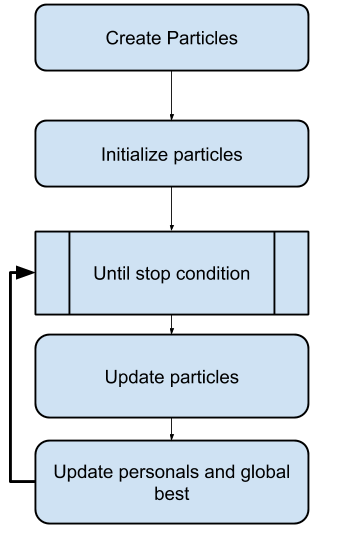
\includegraphics[width=1.5in,height=2.5in]{_img/img_PSO_algorithm_cpu.png}
\caption{PSO cpu implementation}
\end{figure}

\begin{figure}[H]
\centering
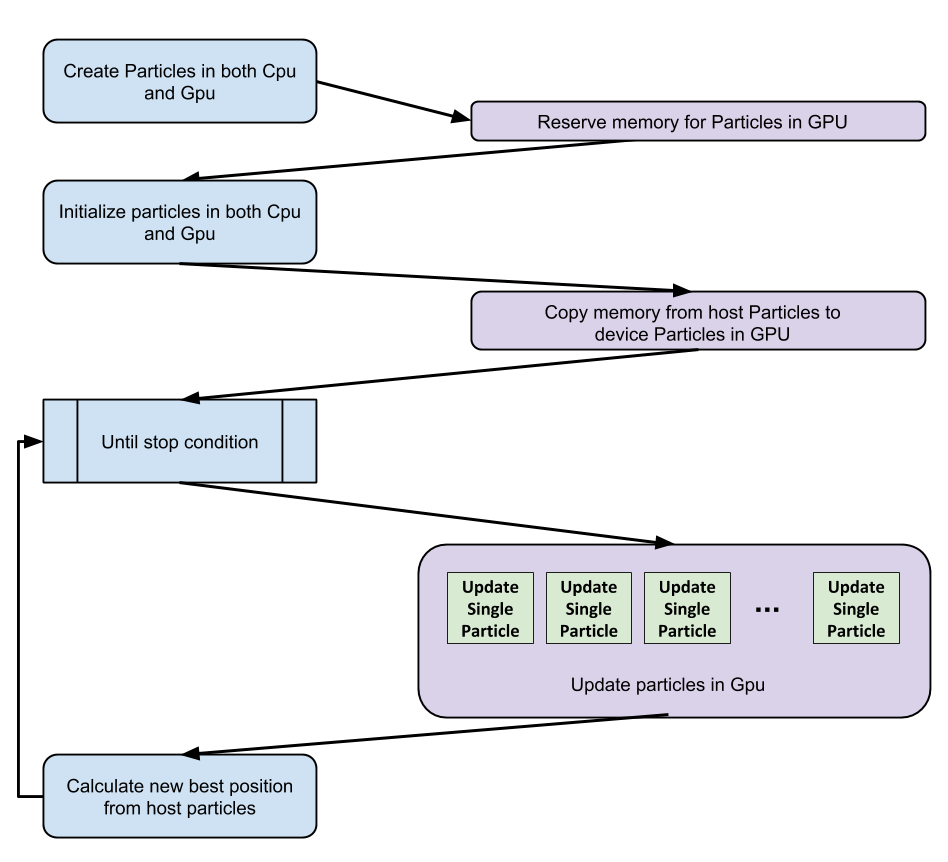
\includegraphics[width=3.5in,height=3.5in]{_img/img_PSO_algorithm_gpu.png}
\caption{PSO gpu implementation}
\end{figure}

\section{Results}

To test our implementation, we used the following benchmark functions :

\begin{enumerate}
    \item \textbf{Ackley}: This is a function with a minimum global optima at $\textbf{X} = (0,0,\hdots)$ with cost of $0.0$.

    \begin{figure}[H]
    \centering
    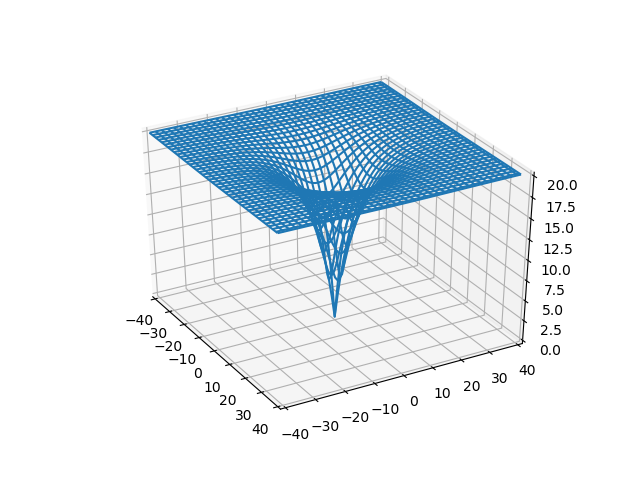
\includegraphics[width=3.0in]{_img/img_bmfunction_ackley.png}
    \caption{Ackley benchmark function}
    \end{figure}

    \item \textbf{Schwefel}: This is a function with a minimum global optima at $\textbf{X} = (420.9687,420.9687    ,\hdots)$ with cost of $0.0$.

    \begin{figure}[H]
    \centering
    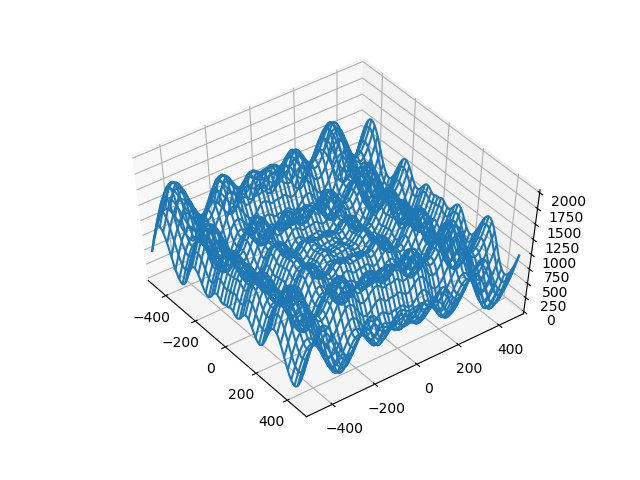
\includegraphics[width=3.0in]{_img/img_bmfunction_schwefel.jpeg}
    \caption{Schwefel benchmark function}
    \end{figure}

    \item \textbf{Schaffer6}: This is a function with a maximum optima at $\textbf{X} = (0,0,\hdots)$ with cost of $1.0$.

    \begin{figure}[H]
    \centering
    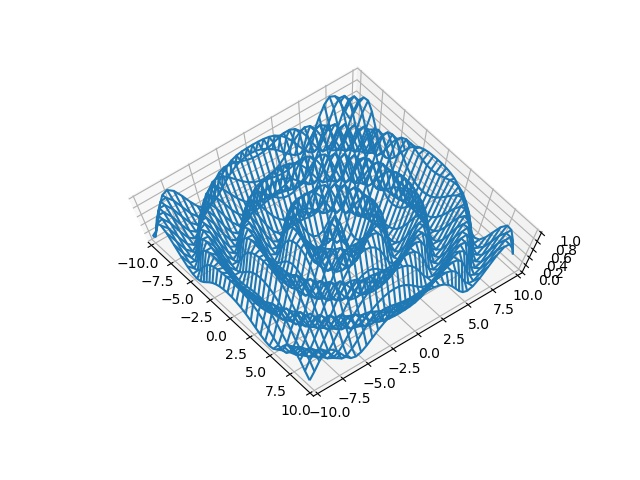
\includegraphics[width=3.0in]{_img/img_bmfunction_schafferfcn6.jpeg}
    \caption{Schaffer6 benchmark function}
    \end{figure}

\end{enumerate}

\begin{figure*}
\centering
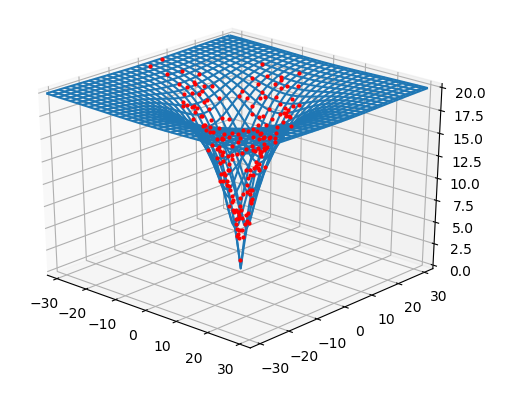
\includegraphics[width=3.0in]{_img/img_PSO_test_2d_ackley_3dview.png}
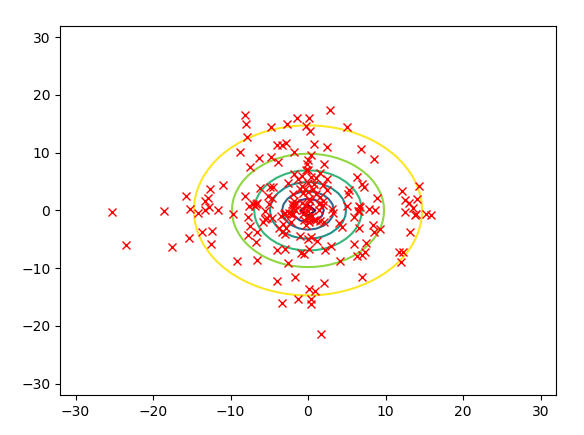
\includegraphics[width=3.0in]{_img/img_PSO_test_2d_ackley_contours.png}
\caption{PSO overview}
\end{figure*}

\begin{figure*}
\centering
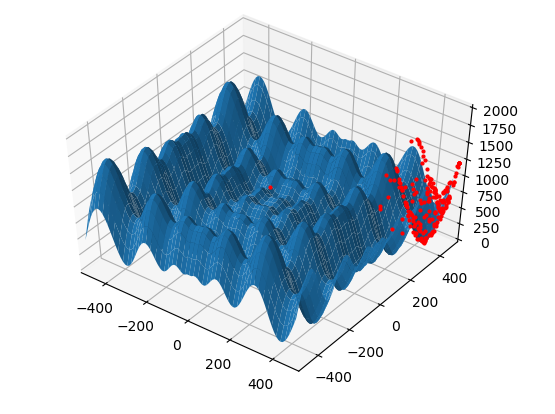
\includegraphics[width=3.0in]{_img/img_PSO_test_2d_schwefel_3dview.png}
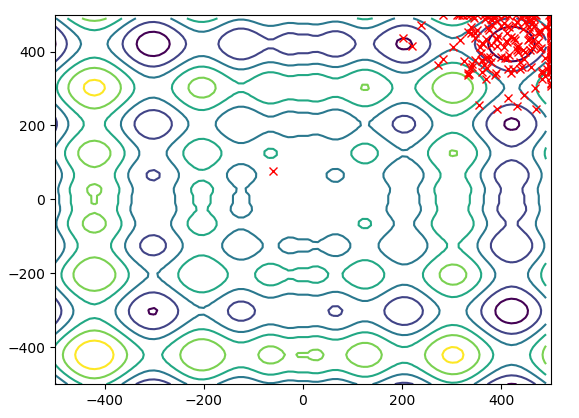
\includegraphics[width=3.0in]{_img/img_PSO_test_2d_schwefel_contours.png}
\caption{PSO overview}
\end{figure*}

\begin{figure*}
\centering
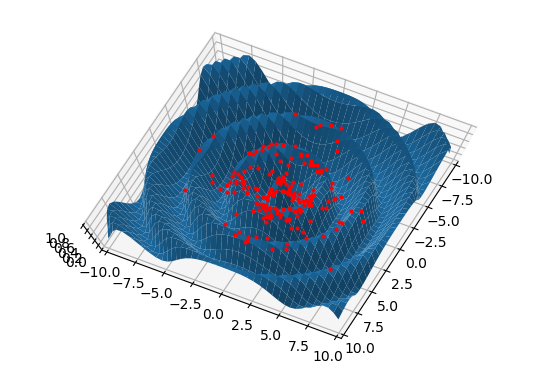
\includegraphics[width=3.0in]{_img/img_PSO_test_2d_schafferfcn6_3dview.png}
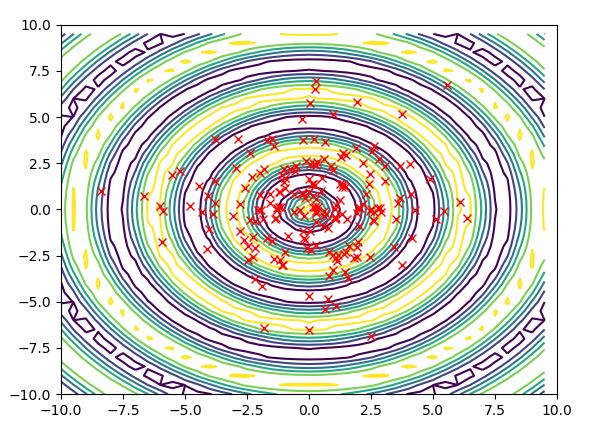
\includegraphics[width=3.0in]{_img/img_PSO_test_2d_schafferfcn6_contours.png}
\caption{PSO overview}
\end{figure*}

\section{Conclusions and Future improvements}



\IEEEtriggeratref{8}

% references section
\begin{thebibliography}{1}

\bibitem{Kennedy1995}
  James Kennedy and Russell Eberhart. \\
  \textit{Particle Swarm Optimization.} - 1995
\\
\bibitem{Garnier2007}
  Simon Garnier, Jacques Gautrais, Guy Theraulaz\\
  \textit{The biological principles of swarm intelligence.} - 2007
\\
\bibitem{delValle2008}
  Yamille del Valle, Ganesh Kumar, Salman Mohagheghi, Jean Hernandez, Ronald Harley\\
  \textit{Particle Swarm Optimization: Basic Concepts, Variants and Applications in Power Systems.} - 2008
\\
\bibitem{CameraCalibration1}
  Zhengyou Zhang \\
  \textit{A Flexible New Technique for Camera Calibration.} - 2000
\\
\bibitem{IntegralImageThresholding}
  Derek Bradley, Gerhard Roth \\
  \textit{Adaptive Thresholding Using the Integral Image.} - 2011

\end{thebibliography}

\section{Appendix}

\begin{algorithm*}
    \caption{Particle Swarm Optimization - Asynchonous Serial Version}\label{alg:PSOcpu}
    \begin{algorithmic}[1]
        \State $\textbf{In}: \textit{objFunction, populationSize, w, $c_{1}$, $c_{2}$, k, dimensions, domain}$
        \State $\textbf{Out}: \textit{Solution optima } P_{g.cost}$
        \State $vMin = -k * ( domain.max - domain.min ) / 2.0$
        \State $vMax =  k * ( domain.max - domain.min ) / 2.0$
        \State $P_{g.pos} = \textit{zeros( dimensions )}$ \Comment{Position that gives best cost}
        \State $P_{g.cost} = Inf$ \Comment{Best cost so far}
        \\
        \State $Particles=\lbrace \rbrace$ \Comment{Empty array of particles}
        \For {$i=1$ {\bfseries to} $PopulationSize$} \Comment{Particles Initialization}
            \State $p = \textbf{Particle()}$
            \State $p.pos = \textbf{randUniform( domain )}$
            \State $p.vel = \textbf{zeros( dimensions )}$
            \State $p.cost = \textbf{objFunction( p.pos )}$
            \State $p.bestpos = p.pos$
            \State $p.bestcost = p.cost$
            \If {$p.cost \leq P_{g.cost}$}
                \State $P_{g.cost} = p.cost$
                \State $P_{g.pos} = p.pos$
            \EndIf
        \EndFor
        \\
        \While {$\textit{ !stopCondition() }$} \Comment{Optimization process}
            \For {$p$ {\bfseries in} $Particles$}
                \State $p.vel = w * p.vel + 
                                c_{1} * ( p.bestpos - p.pos ) + 
                                c_{2} * ( P_{g.pos} - p.pos )$ \Comment{Velocity update}
                \State $p.vel = \textbf{ClampVector}\textit{( p.vel, vMin, vMax )}$
                \State $p.pos = p.pos + p.vel$ \Comment{Position update}
                \State $p.pos = \textbf{ClipPosition}\textit{( p.pos, domain )}$
                \\
                \If {$p.cost \leq p.bestcost$}
                    \State $p.bestcost = p.cost$ \Comment{Update personal best}
                    \State $p.bestpos = p.pos$
                    \If {$p.cost \leq P_{g.cost}$}
                        \State $P_{g.cost} = p.cost$ \Comment{Update global best}
                        \State $P_{g.pos} = p.pos$
                    \EndIf
                \EndIf
            \EndFor
        \EndWhile
        \\
        \Return $P_{g.cost}$
    \end{algorithmic}
\end{algorithm*}

\begin{algorithm*}
    \caption{Particle Swarm Optimization - Synchonous Parallel Gpu Version}\label{alg:PSOgpu}
    \begin{algorithmic}[1]
        \State $\textbf{In}: \textit{objFunction, populationSize, w, $c_{1}$, $c_{2}$, k, dimensions, domain}$
        \State $\textbf{Out}: \textit{Solution optima } P_{g.cost}$
        \State $vMin = -k * ( domain.max - domain.min ) / 2.0$
        \State $vMax =  k * ( domain.max - domain.min ) / 2.0$
        \State $P_{g.pos} = \textit{zeros( dimensions )}$ \Comment{Position that gives best cost}
        \State $P_{g.cost} = Inf$ \Comment{Best cost so far}
        \\
        \State $hostParticles = \lbrace \rbrace$
        \State $deviceParticles = \lbrace \rbrace$
        \State $\textbf{GpuCreateParticles}\textit{( hostParticles, deviceParticles, objFunction, populationSize, dimensions, domain )}$
        \State $\textbf{GpuInitParticles}\textit{( hostParticles, deviceParticles, objFunction )}$
        \\
        \While {$\textit{ !stopCondition() }$} \Comment{Optimization process}
            \State $\textbf{GpuUpdateParticles}\textit{( hostParticles, deviceParticles, w, $c_{1}$, $c_{2}$, k )}$s
            \For {$p$ {\bfseries in} $hostParticles$}
                \If {$p.cost \leq P_{g.cost}$}
                    \State $P_{g.cost} = p.cost$ \Comment{Update global best}
                    \State $P_{g.pos} = p.pos$
                \EndIf
            \EndFor
        \EndWhile
        \Return $P_{g.cost}$
    \end{algorithmic}
\end{algorithm*}

\begin{algorithm*}
    \caption{Particle Swarm Optimization - GpuUpdateParticles}\label{alg:PSOgpu_kernel_updateparticles}
    \begin{algorithmic}[1]
        \State $\textbf{In}: \textit{deviceParticles, coreIndx, w, $c_{1}$, $c_{2}$, k, $P_{g}$}$
        \State $p = \textbf{getDeviceParticle}\textit{( coreIndx )}$
        \State $p.vel = w * p.vel + 
                        c_{1} * ( p.bestpos - p.pos ) + 
                        c_{2} * ( P_{g.pos} - p.pos )$ \Comment{Velocity update}
        \State $p.vel = \textbf{ClampVector}\textit{( p.vel, vMin, vMax )}$
        \State $p.pos = p.pos + p.vel$ \Comment{Position update}
        \State $p.pos = \textbf{ClipPosition}\textit{( p.pos, domain )}$
        \\
        \If {$p.cost \leq p.bestcost$}
            \State $p.bestcost = p.cost$ \Comment{Update personal best}
            \State $p.bestpos = p.pos$
        \EndIf
    \end{algorithmic}
\end{algorithm*}


\end{document}
